\documentclass{beamer}
\usepackage{graphicx}
\usepackage{xeCJK}
\setCJKmainfont{WenQuanYi Zen Hei}
\usetheme{Frankfurt}
\useinnertheme{circles}
\hypersetup{colorlinks=true,linkcolor=red}
\begin{document}
{
\begin{frame}
    \title{文献阅读:{\color{red}{A high-resolution map of human evolutionary constraint using 29 mammals}}}
    \author{元件注释}
    \institute{BGI-RD\\深圳}
    \maketitle
\end{frame}
}

\begin{frame}{Outline}                       %contents only page !
\tableofcontents
\end{frame}
%%-------------------------
\begin{frame}{研究背景}
%如果控制颜色的花括号不空行的话会被latex当成是标题的次标题,这时使不能加双斜线断行的,空行之后就没有误会,可以断行了

{\color{red}{已知:}}\\
人类基因组中编码部分约1.5\%,HMRD表明5\%受到purifying selection,其中又~3.5\%是非编码元件,可能与基因调控相关。\\
{\color{red}{已有研究:}}
\begin{itemize}				
\item HMRD:human-mouse-rat-dog
\item Sipel:vertebrate 
\end{itemize}
之前的比较基因组研究确定了这部分区域大体含量,但是不能检测到具体的constraint element,因为分辨率不够,所以之前的工作只是针对5\%中最保守的top 5\%。
\end{frame}

\begin{frame}{本文工作}
自2005年为29哺乳动物测序,以人类基因组做参考,确定高分辨率的map,希望找到并细致分析保守元件。
\begin{itemize}
\item 肯定了之前关于保守元件约占总量5\%的估计
\item 确定了4.2\%的序列是保守的,利用多种证据确定了其中60\%是功能相关的
	\begin{itemize}
	\item	protein-coding 
	\item RNA
	\item 调控区和chromatin roles
	\end{itemize}
\item 提供了exaptation 和加速进化的证据
\end{itemize}
{\color{red}{Expation}}:在进化过程中一些特征改变了最初的功能 -by Gould\\
$$http://en.wikipedia.org/wiki/Exaptation$$								
\end{frame}
					
\begin{frame}{sequencing,asembly and alignment}
\begin{itemize}
\item 7-fold:9  species previously described
\item 2-fold:20 species first reported

20species 质量统计:
\begin{itemize}
\item contig size $N50_c$ :2.8kb 
\item scaffold size $N50_s$ :51.8kb 
\item 96\% had quality score $Q_{20}$,corresponding to a <1\% error rate
\end{itemize}
\end{frame}

\begin{frame}{sequencing,asembly and alignment}
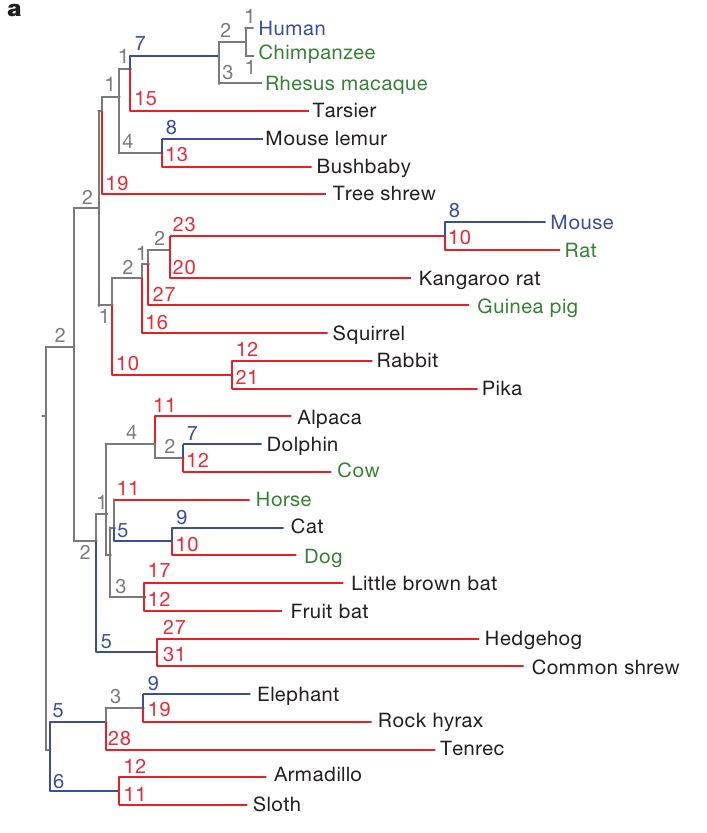
\includegraphics[width=8cm,angle=-90]{../clade.png}
\end{frame}

\begin{frame}{sequencing,asembly and alignment}
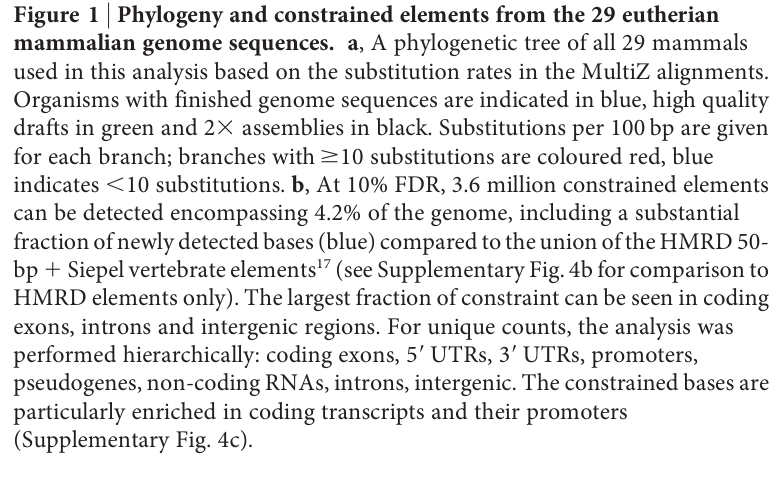
\includegraphics[width=10cm]{../clade_notes.png}
\end{frame}

\begin{frame}{sequencing,asembly and alignment}
增加了物种间的差异,枝长显著增加。
\begin{itemize}
\item HMRD:0.68 substitution per site
\item 20Ma:4.5  substitution per site
\end{itemize}
检验保守元件的能力主要取决于进化树的总枝长:the power to detect constrained elements depends largely on the total branch length of the phylogenetic tree connection the species.\\
Cooper,G.M, {\color{red}{A quantitive estimates of sequence divergence for comparative analysis of mammaliang genomes}}
\end{frame}
\end{document}

